\chapter{Background and Related Work}
In this chapter, we first discuss different approaches to text representation including encoding documents as \textit{Bag of Words}, creating word vectors using word embedding technique \textit{word2vec}, related algorithm for creating paragraph vectors \textit{doc2vec}. We close the section with recurrent and convolutional network approaches to text classification. In the following, we mention few classification algorithms we use for the genre prediction and introduce \textit{Project Gutenberg} - an online repository of books, which is the source of our datasets.


\section{Classification}
\label{classification_algorithms}

\begin{itemize}
    \item introduction to this section
\end{itemize}

\subsection{Classification problem definition}
\begin{itemize}
    \item what is a classification (define classification problem)
    \item feature vector, label
\end{itemize}

\subsection{Evaluation metrics}
\begin{itemize}
    \item two classes vs. multiple classes
\end{itemize}

\subsubsection{Accuracy}
\smallskip
\subsubsection{Precision, Recall and F1-score}
\smallskip


\subsection{Distance metric and similarity}
\subsubsection{l1 \& l2 metric}
\smallskip
\subsubsection{Cosine similarity}
\smallskip

\subsection{Hyperparameter optimization}
\begin{itemize}
    \item regularization
    \item K-fold cross-validation
    \item Grid Search
    \item Random Search
\end{itemize}

\section{Classification Algorithms}

\subsection{Naive Bayes classifier}
\smallskip

\subsection{Logistic Regression}
\begin{itemize}
    \item $x^{(i)}$ - i-th datapoint (vector)
    \item $y^{(i)}$ - label $\in \{0, 1\}$ of the $i$-th datapoint
    \item $\theta$ - vector of model coefficients
    \item $h_\theta(x)$ - prediction for $x$ given a vector of coefficients $\theta$
    \item $m$ - number of samples
    \item $n$ - number of features
    \item $J(\theta)$ - loss function for given $\theta$ which is to be minimized
\end{itemize}

Prediction for vector $x$:
$$h_{\theta} (x) = \frac{1}{1 + e^{-\theta^T x}}$$

Loss function:
$$J(\theta) = -\frac{1}{m} \sum_{i = 1}^{m}[y^{(i)}log(h_\theta(x^{(i)})) + (1-y^{(i)})log(1-h_\theta(x^{(i)}))] + \frac{\alpha}{2m}\sum_{j=1}^n \theta_j^2$$

\subsection{Feed-forward neural network}
\smallskip
\subsubsection{Activation Functions}
\begin{itemize}
    \item RelU
    \item Sigmoid
    \item Softmax
\end{itemize}

\subsubsection{Dropout Layer}
Dropout\cite{dropout1}\cite{dropout2} is a regularization technique which prevents complex co-adaptations on the training set and hence reduces overfitting. Dropout layer can be put between two layers of the neural net and it drops (sets to zero) a neuron going into it with a given dropout rate $p$.

The higher the dropout rate, the more iterations are needed to train the network. If the dropout rate is set too high, the net might underfit the training data.

\section{Text Analysis}
\label{text_analysis}

Typical text analysis tasks are classifying texts into given categories or adding tags. Recently, the research moves towards tasks related to human perception of the text. One of those is \textit{sentiment analysis} where the goal is to determine writer's attitude. For example, we might be interested in determining if a review of a product is positive or negative. Another popular task is recognizing fake news.[CITE]

Based on the task, different approaches are needed. For genre classification, both sentences
\begin{itemize}
    \item He looked at the detective.
    \item He didn't look at the detective.
\end{itemize}
probably come from a detective story. The genre does not depend on if the word \textit{look} is in a positive or negative context. The individual word choice is more important. In that case, bag of word approaches (with tf-idf term weighting) perform usually good.[CITE]

On the other hand, in case of sentiment analysis, two sentences
\begin{itemize}
    \item I didn't enjoy the movie.
    \item I didn't enjoy the movie at first.
\end{itemize}
capture different sentiment as in the second case, the writer implies they liked the movie after all. To capture these nuances, the model has to keep the context of the whole sentence, which is one of the reasons neural networks with LSTMs or convolution windows win in these tasks.[CITE]

glossary:
\begin{itemize}
    \item corpus
    \item document
    \item class (e.g. genre, positive sentiment etc.)
\end{itemize}

\subsection{Bag of Words}
First representation we explore is Bag of Words (BOW), which has been proved [CITE] to be a decent baseline for text classification tasks. In BOW, each document is represented by a vector of zeros and ones. The length of the vector is given by the size of \textit{vocabulary} - list of words of interest. The $j$-th component of the BOW vector $v_i$ corresponding to the $i$-th document of the corpus is then defined as follows: 
$$
  v_{ij} = \left\{\begin{array}{ll}
      1, & \text{if } j \text{-th word of the vocabulary occurs in the }i \text{-th document}\\
      0, & \text{otherwise}\\
      \end{array}\right\}
$$

To keep the vocabulary meaningful, it is common to drop words with both very high and very low occurrence. Frequent words usually don't carry any meaning nor significance to the predicted classes. These words are also called \textit{stop-words} and it is common practice to filter them out of the texts. Keeping the low-occurrence words might introduce noise into vocabulary where the added words are not typical for the given class, just happened to be seen in a document. Therefore, only words that occur in more than $d$ documents are added to vocabulary.

The filtering is highly dependent on the corpus. If all documents are novels, the word \textit{you} probably won't help much in classification. However, if the goal is to distinguish novels from news articles, the word \textit{you} could be worth keeping.

\begin{itemize}
    \item popular for spam detection[CITE]
    \item introduce the word vocabulary
\end{itemize}



\begin{comment}
\subsubsection{Tf-Idf}
\subsubsection{Part of Speech}
\subsubsection{Stemming \& Lemmatization}
\subsubsection{Stop Words}
\subsubsection{N-grams}
\end{comment}



\subsection{Word2Vec}
\begin{itemize}
    \item Representative of word-embeddings.
    \item First published approach of its type to word embeddings.
    \item other embeddings - GloVe\cite{glove}, Fasttext\cite{fasttext}
\end{itemize}

\begin{comment}
GloVe - Wikipedia 2014 + Gigaword 5
\end{comment}


Explain word2vec\cite{word2vec} and the two approaches:
\begin{itemize}
    \item continuous bag of words (CBOW) (\cref{fig:word2vec_skip_gram})
    \item skip gram
\end{itemize}

\begin{figure}[h]
	\centering
	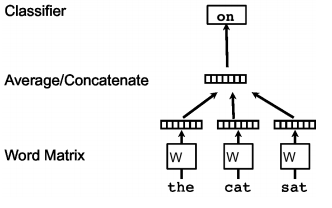
\includegraphics[height=0.2\textheight]{img/word2vec_skip_gram}
    \caption{Word2vec -- Skip gram architecture\cite{doc2vec}}
    \label{fig:word2vec_skip_gram}
\end{figure}

Other things to mention:
\begin{itemize}
    \item show 2D projection of vectors
    \item $king + woman - man = queen$
\end{itemize}

\subsection{Paragraph Vector (Doc2Vec)}
Explain doc2vec\cite{doc2vec}.

\begin{comment}
dbow
is a simpler model and ignores
word order, while
dmpv
is a more complex model
with more parameters

dbow 
works in the same way as skip-gram, except that the input is replaced by a special token representing the document (i.e. v_w_I is a vector rep-
resenting the document).  In this architecture, the order of words in the document is ignored; hence the name distributed bag of words.

dmpv
works in a similar way to cbow. For the input, dmpv introduces  an  additional  document token  in  addition  to  multiple  target  words. Unlike cbow, however, these vectors are not summed but concatenated (i.e.
v_w_I is a concatenated vector containing the document token and several target words). The objective is again to predict a context word given the concatenated document and word vectors..

\end{comment}

\begin{itemize}
    \item distributed memory version (dm) (\cref{fig:doc2vec_dm})
      \subitem small extension to cbow word2vec
      \subitem acts as a memory - what is missing from the current context?
    \item distributed bag of words (dbow) (\cref{fig:doc2vec_dbow})
      \subitem similar to skip-grams in word2vec
\end{itemize}

\begin{figure}[h]
	\centering
	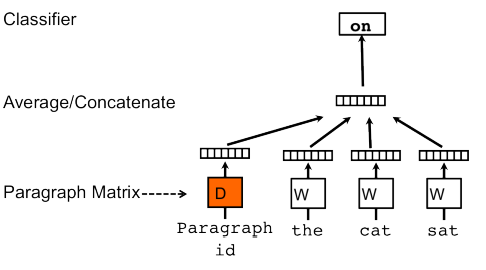
\includegraphics[height=0.2\textheight]{img/doc2vec_dm}
    \caption{Paragraph Vector -- Distributed Memory version\cite{doc2vec}}
    \label{fig:doc2vec_dm}
\end{figure}

\begin{figure}[h]
	\centering
	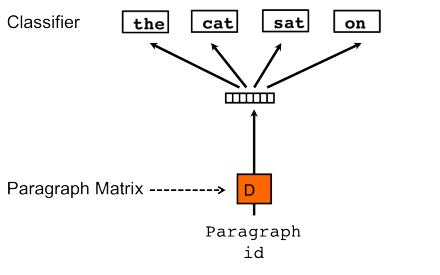
\includegraphics[height=0.2\textheight]{img/doc2vec_dbow}
	\caption{Paragraph Vector -- Distributed Bag of Words version\cite{doc2vec}}
	\label{fig:doc2vec_dbow}
\end{figure}

\subsection{Deep Learning}
deep learning\cite{Goodfellow}

Input - sequence of word embeddings.

\subsubsection{Recurrent Neural Network (RNN)}
\begin{itemize}
    \item cite relevant papers
    \item put an image of the network
    \item LSTM units
\end{itemize}

\subsubsection{Convolutional Neural Networks}
Show Yoon Kim's\cite{yoon_kim} architecture (\cref{fig:cnn_kim}).


Mention Zhang.\cite{cnn_zhang}.

\begin{figure}[h]
	\centering
	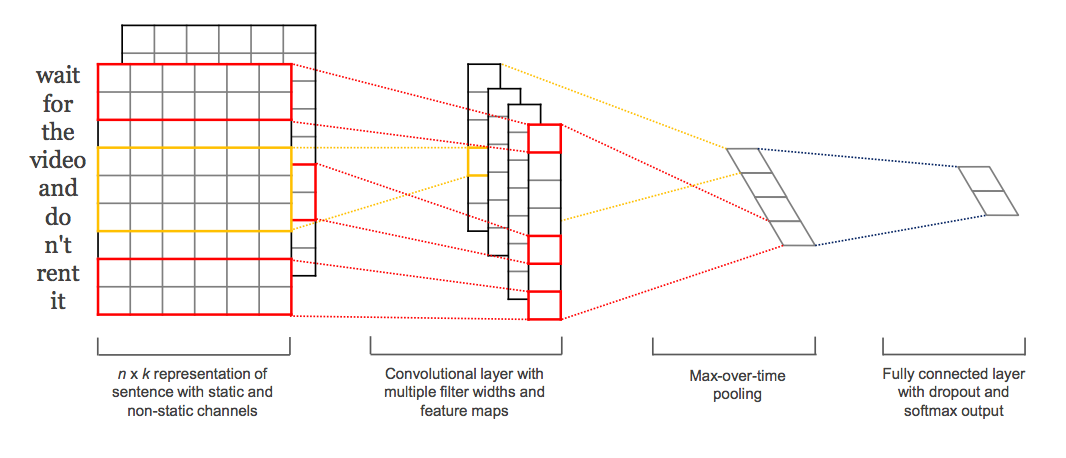
\includegraphics[height=0.2\textheight]{img/cnn_kim}
	\caption{Convolutional neural network with multiple filter sizes\cite{yoon_kim}}
	\label{fig:cnn_kim}
\end{figure}


%%%%%%%%%%%%%%%%%%%%%%%%%%%%%
%%%%%%%%% BOOSTING %%%%%%%%%%
%%%%%%%%%%%%%%%%%%%%%%%%%%%%%
\begin{comment}

\begin{itemize}
    \item Random Forest
    \item XGBoost
    \item stacking
\end{itemize}
\end{comment}



\begin{comment}
\subsection{Annoy}
Annoy\cite{annoy} is a algorithm developed by Erik Bernhardsson at Spotify, which enables quick search for the nearest neighbours. The drawback of the traditional kNN algorithm is its linear prediction time and huge amount of memory needed, which doesn't scale once we have hundreds of thousands data points.

Annoy uses random projections and recursively splits the space between two data points by a random hyperplane. All the splits are stored in the tree. The whole algorithm is run $n$ times to create $n$ trees. The more trees, the better the accuracy and slower the training and prediction time.
\end{comment}

\section{Project Gutenberg}
\begin{itemize}
    \item What is Project Gutenberg.
    \item How many books are there in Project Gutenberg
    \item What types (classes) of books
    \item Metadata for genre classification.
\end{itemize}
